\section{Belgian energy system in 2020} 
\label{app:bel_2020}
The Belgian whole-energy system of 2020 was largely based (88.6\% of the primary energy mix) on \og conventional fuels\fg (\ie oil and oil products (38.2\%), natural gas (29.5\%), uranium (16.3\%) and solid fossil fuels (4.6\%) while the rest mainly accounts for 26.7\,TWh of lignocellulosic and wet biomass, 12.8\,TWh of wind and 5.1\,TWh of solar \cite{spf_economy_2022}. Given the data available in the literature (mostly for the power sector) and, when not available, following the assumptions made by \citet{Limpens2020}, \Cref{tab:Belgium_2020} gives the major technologies used in 2020 to supply the different demands of \Cref{fig:cs_demands}.

\begin{table}[htbp!]
\caption{Major technologies used to supply the 2020-demands of \Cref{fig:cs_demands} in terms of share of production and installed capacity.}
\label{tab:Belgium_2020}
\begin{minipage}{\linewidth}
\centering
\resizebox{\textwidth}{!}{
\begin{tabular}{l c c c}
\toprule
\multirow{2}{*}{\textbf{End-use demand}} & \textbf{Major} & \textbf{Share of} & \textbf{Installed}\\
    &	 \textbf{technologies} 	& \textbf{supply} & \textbf{capacity}	 \\ 	
\midrule							
\multirow{3}{*}{Electricity}
 & Nuclear & 39\% & 5.9\,GW\\
 & CCGT & 21\% & 3.9\,GW\\
 & Wind turbines & 14\% & 5.0\,GW\\
\midrule
\multirow{3}{*}{Heat High-Temp.}
 & Gas boiler & 36\% & 3.3\,GW\\
 & Coal boiler & 30\% & 2.3\,GW\\
 & Oil boiler & 20\% & 1.5\,GW\\
\midrule
\multirow{3}{*}{Heat Low-Temp. (DEC)\footnote{\label{foot:DHN_98}The decentralised heating units provide 98\% of the low-temperature heat demand. }}
 & Oil boiler & 48\% & 21.4\,GW\\
 & Gas boiler & 40\% & 17.5\,GW\\
 & Wood boiler & 10\% & 4.4\,GW\\
\midrule
\multirow{3}{*}{Heat Low-Temp. (DHN)}
 & Gas CHP & 59\% & 0.3\,GW\\
 & Gas boiler & 15\% & 0.3\,GW\\
 & Waste CHP & 15\% & 0.1\,GW\\
\midrule
\multirow{2}{*}{Private mobility\footnote{\label{foot:privatemob_80}The private mobility accounts for 80\% of the passengers mobility.}}
 & Diesel car & 49\% & 93.5\,Mpass.-km/h\\
 & Gasoline car & 49\% & 94.7\,Mpass.-km/h\\
 & HEV & 2\% & 5.9\,Mpass.-km/h\\
\midrule
\multirow{3}{*}{Public mobility}
 & Diesel bus & 43\% & 3.6\,Mpass.-km/h\\
 & Train & 43\% & 3.9\,Mpass.-km/h\\
 & CNG bus & 5\% & 0.8\,Mpass.-km/h\\
\midrule
\multirow{3}{*}{Freight mobility}
 & Diesel truck & 74\% & 62.7\,Mt.-km/h\\
 & Diesel boat & 15\% & 10.8\,Mt.-km/h\\
 & Train & 11\% & 2.5\,Mt.-km/h\\
\midrule
HVC & Naphtha/LPG cracking & 100\% & 4.6\,GW\\
Ammonia & Haber-Bosch & 100\% & 1\,GW\\
Methanol & Import & 100\% & -\\
\bottomrule							
\end{tabular}}
\end{minipage}
\end{table}

\section{\ce{CO2}-budget versus linear decrease of emissions}
\label{app:CO2_budget}

\Cref{fig:app_CO2_REF_lin} shows the yearly emissions attributed for each sector in the REF case (\ie imposed \ce{CO2}-budget) and a case where the \ce{CO2}-trajectory is constrained instead. Interestingly, these two transition pathways end up in a similar carbon-neutral whole-energy system in 2050. The two main sectors that significantly reduce their emissions in the REF case are the production of \gls{HVC} and the high-temperature heat. In the former, this is linked to the extended use of oil products through naphtha-cracking. The latter is produced by industrial coal boilers for longer, until 2040. Overall, ending up to the same level of emissions in 2050, the REF case represents a 60\% reduction of the cumulative emissions compared to the linear decrease, for a 7.5\% more expensive transition.

\begin{figure}[htbp!]
\centering
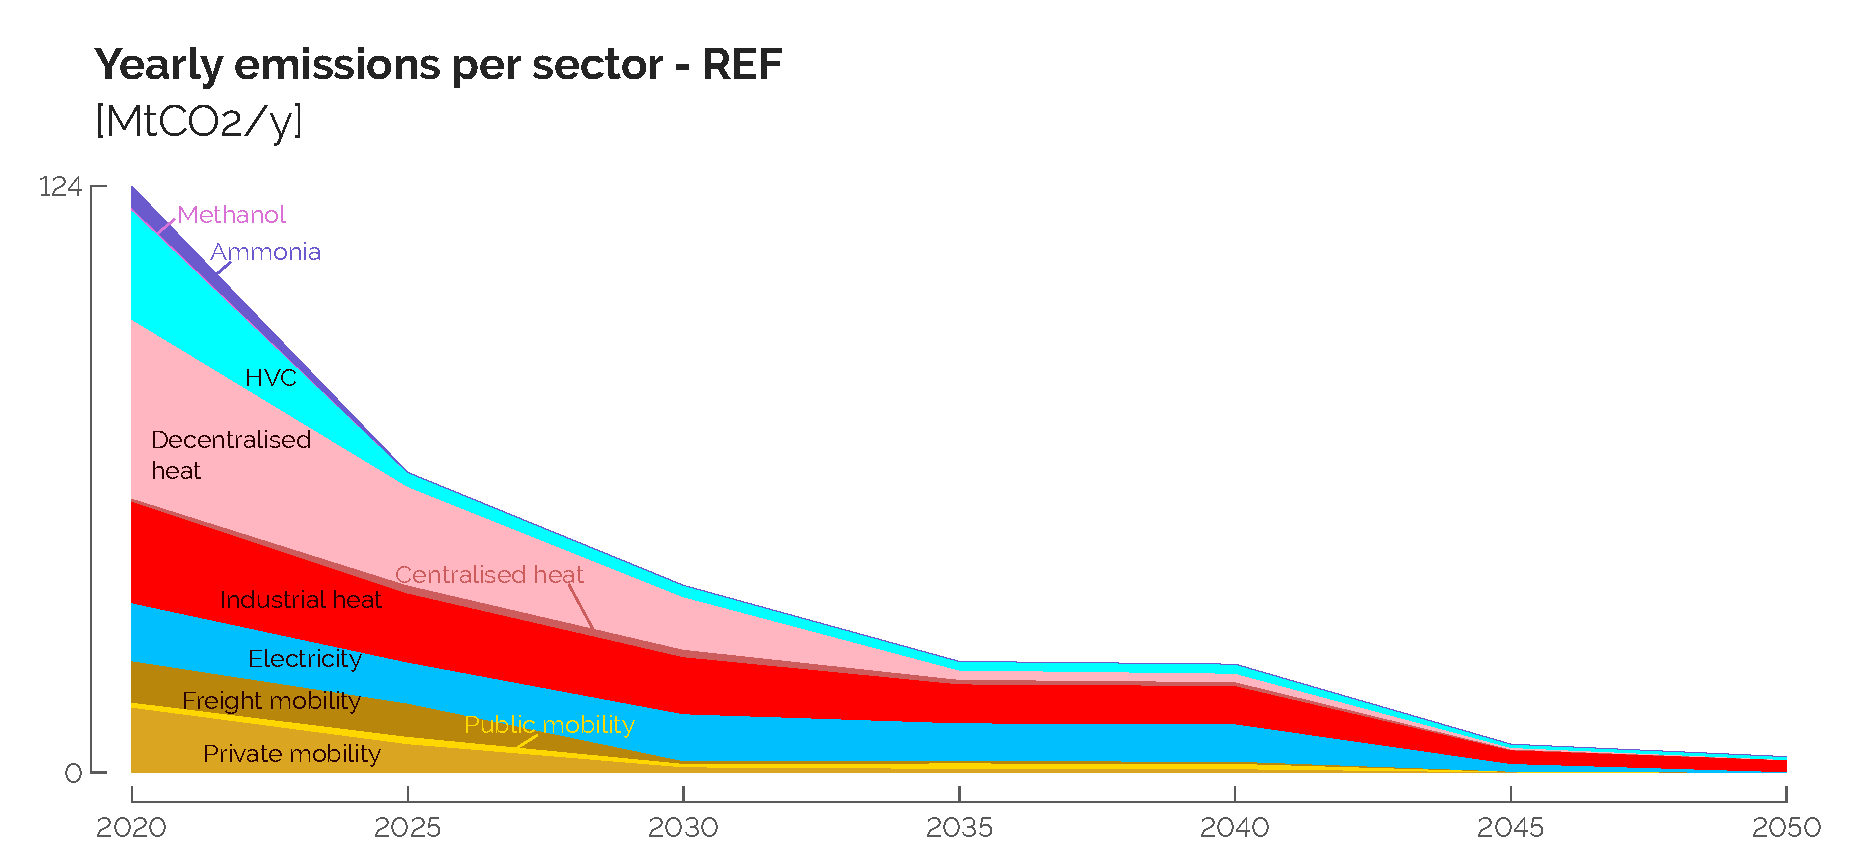
\includegraphics[width=0.49\textwidth]{GWP_per_sector_REF.pdf}
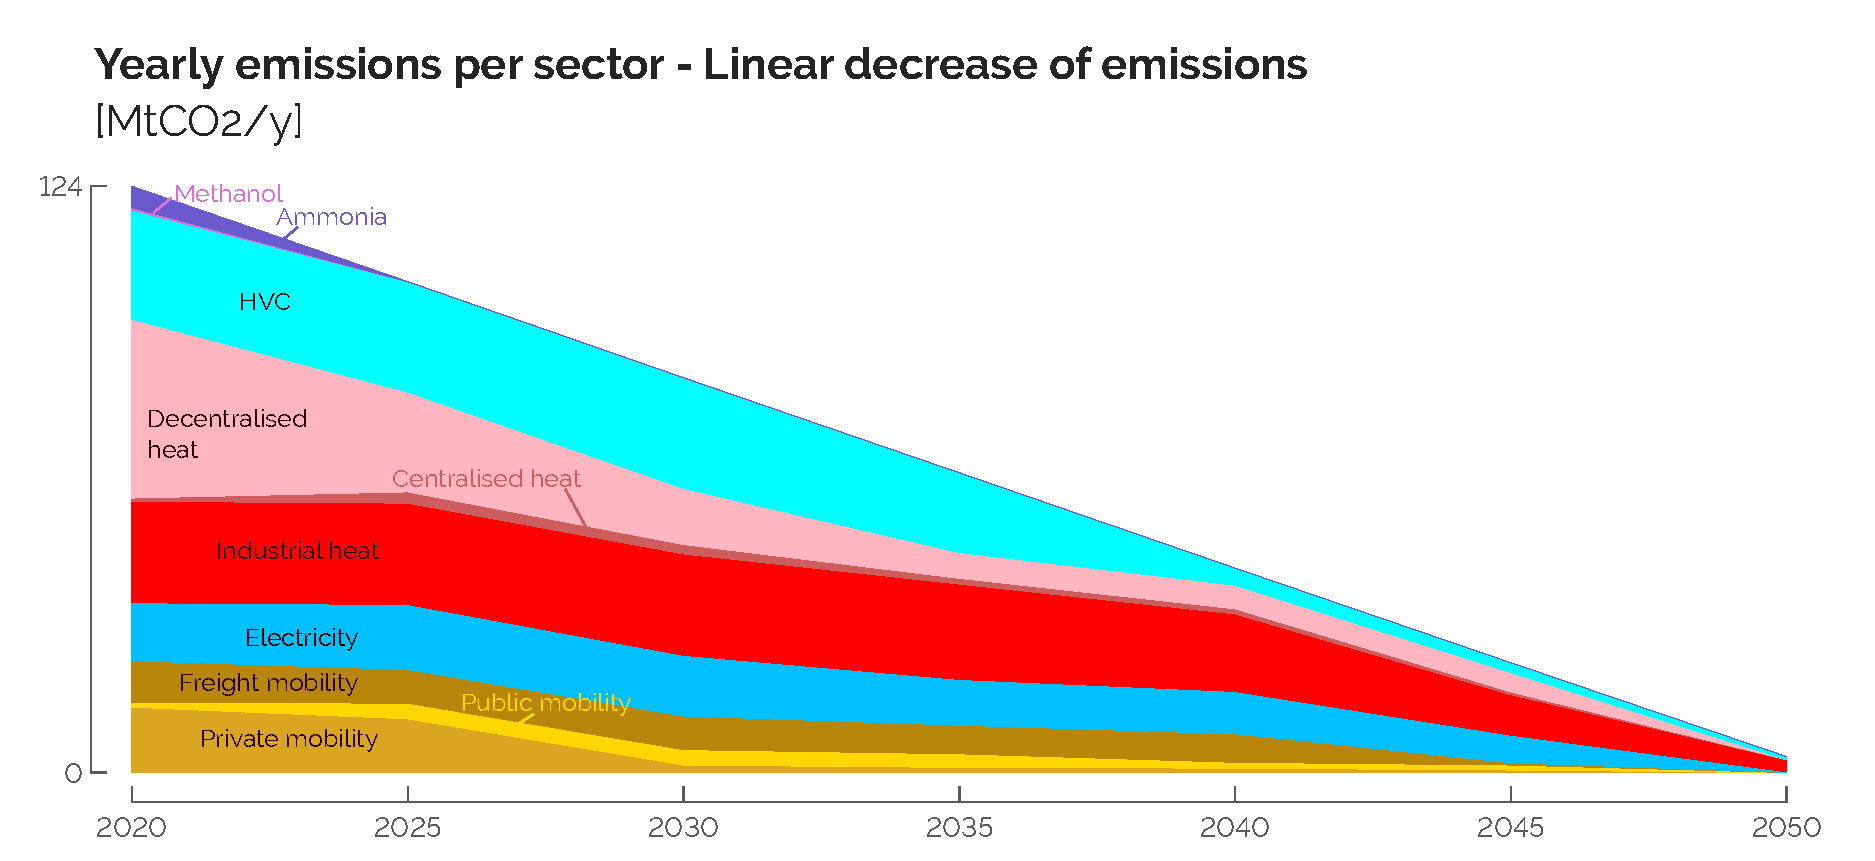
\includegraphics[width=0.49\textwidth]{GWP_per_sector_lin.pdf}
\caption{Respecting the \ce{CO2}-budget imposed in the REF case drastically cuts the emissions of the system, especially in the production of \glsxtrfull{HVC} and the high-temperature heating sector.}
\label{fig:app_CO2_REF_lin}
\end{figure}

\section{Uncertainty characterisation for the 5-year steps transition} 
\label{app:UC_full}
Table \ref{tab:UC_full} summarises the uncertainty ranges for the different groups of technologies and resources, for the year 2025. Refer to \cite{Moret2017, Moret2017PhDThesis} for the methodology and sources. As the model optimises the system every 5 years, $N=5$ has been selected to get the final ranges of uncertainties of type II and III, based on the work of \citet{Moret2017PhDThesis}. For type III uncertainties (\ie uncertainty ranges increasing with time), a 50\% increase has been set arbitrarily between the ranges for 2025 and these same ranges for 2050. In other words, for these specific uncertainties, the ranges for 2050 are 50\% larger than for 2025.

\citet{rixhon2021role} analysed the impact of these parameters on the total cost of the snapshot Belgian whole-energy system in 2050 subject to different \gls{GWP} limits. Based on this work, we have selected a subset of impacting uncertainties, added others due to the pathway formulation (\eg $\Delta_{\mathrm{change,pass}}$), and listed them in Table \ref{tab:UC_full}. The uncertainty characterisation gives the uncertainty ranges per parameter or group of parameters (category).

This work considers nine groups of uncertain parameters: (i) the cost of purchasing imported energy carriers; (ii) the investment cost (\ie CAPEX) of some technologies, mostly related to the mobility sector and the integration of renewables; (iii) the maintenance cost (\ie OPEX) of every technology; (iv) the consumption of electric and fuel cells vehicles in the mobility sector; (v) the potential installed capacity of renewables; (vi) the hourly load factor of renewables accounting for variability of solar irradiance or wind speed; (vii) the availability of resources considered as limited (\ie biomass and electricity); (viii) the end-use-demands split per sector of activities (\ie households, services, passenger mobility and industry) and (ix) other parameters like the interest rate or the modal share change in different key sectors. For the specific case of \gls{SMR}, the parameter $f_{\mathrm{max,SMR}}$ will influence the maximum capacity (\ie 6~GW) to install to translate somehow the readiness of this technology. If it is (i) smaller than 0.6, there is no possibility to install \gls{SMR} during the transition; (ii) between 0.6 and 0.8, these 6~GW can be installed only in 2050; (iii) between 0.8 and 0.9, these can be installed from 2045 onward and; (iv) higher than 0.9, the prescribed maximum capacity can be installed from 2040 onward. 

% \textcolor{red}{\textbf{See low-wind speed in 2021 from energy key data edition february 2023 (wind-based production decreased 6.4\% despite additional wind farm installations), to justify the -22\% for c,p,t}}

%$^{(a)}$ Per \cite{Moret2017PhDThesis}, \og I: investment-type, II: operation-type (constant uncertainty over time), III: operation-type (uncertainty increasing over time)\fg. $^{(b)}$ The nominal values of each of the parameters is 0, meaning no variation compared to the nominal values of the impacted parameter in the model. $^{(c)}$ This range has been inferred from the local sensitivity analysis performed by \citet{PATHS2050}.

\begin{table}[htbp!]
\caption{Application of the uncertainty characterization method to the EnergyScope Pathway model for the year 2025. }
\label{tab:UC_full}
\begin{minipage}{\linewidth}
\centering
\resizebox{\textwidth}{!}{
\begin{tabular}{l l l c c c}
\toprule
\multirow{2}{*}{\textbf{Category}} & \multirow{2}{*}{\textbf{Parameter}} & \multirow{2}{*}{\textbf{Meaning}} & \multirow{2}{*}{\textbf{Type}\footnote{\label{foot:type_uncert_range}Per \cite{Moret2017PhDThesis}, \og I: investment-type, II: operation-type (constant uncertainty over time), III: operation-type (uncertainty increasing over time)\fg . }}  & \multicolumn{2}{c}{\textbf{Relative variation}\footnote{\label{foot:nom_val_uncert}The nominal values of each of the parameters is 0, meaning no variation compared to the nominal values of the impacted parameter in the model. }}\\
    & & & &	 min 	&	 max \\ 	
\midrule		
\multirow{4}{*}{\textbf{Cost of purchasing}} & $c_{\mathrm{op,fossil}}$ & Purchase fossil fuels & II & -64.3\% & 179.8\% \\
& $c_{\mathrm{op,elec}}$ & Purchase electricity & II & -64.3\% & 179.8\% \\
& $\bm{c_{\mathrm{op,electrofuels}}}$ & \textbf{Purchase electrofuels} & \textbf{II} & \textbf{-64.3\%} & \textbf{179.8\%} \\
& $c_{\mathrm{op,biofuels}}$ & Purchase biofuels & II & -64.3\% & 179.8\% \\
\midrule
\multirow{9}{*}{\textbf{Investment cost}} &$c_{\mathrm{inv,car}}$ & CAPEX car  & I & -21.6\% & 25.0\% \\
& $c_{\mathrm{inv,bus}}$ & CAPEX bus & I & -21.6\% & 25.0\% \\
& $c_{\mathrm{inv,ic\_prop}}$ & CAPEX ICE & I & -21.6\% & 25.0\% \\
& $c_{\mathrm{inv,e\_prop}}$ & CAPEX electric motor & I & -39.6\% & 39.6\% \\
& $c_{\mathrm{inv,fc\_prop}}$ & CAPEX fuel cell engine & I & -39.6\% & 39.6\% \\
& $c_{\mathrm{inv,efficiency}}$ & CAPEX efficiency measures & I & -39.3\%  & 39.3\% \\
& $c_{\mathrm{inv,PV}}$ & CAPEX PV & I & -39.6\% & 39.6\% \\
& $c_{\mathrm{inv,grid}}$ & CAPEX power grid & I & -39.3\% & 39.3\% \\
& $c_{\mathrm{inv,grid\_enforce}}$ & CAPEX grid reinforcement & I & -39.3\% & 39.3\% \\
& $\bm{c_{\mathrm{inv,nuclear\_SMR}}}$ & \textbf{CAPEX \gls{SMR}}\footnote{\label{foot:range_SMR}This range has been inferred from the local sensitivity analysis performed by \citet{PATHS2050}.} & \textbf{I} & \textbf{-40.0\%} & \textbf{44.0\%} \\
\midrule
\textbf{Maintenance cost} & $c_{\mathrm{maint,var}}$ & Variable OPEX of technologies & I & -48.2\% & 35.7\% \\
\midrule
\multirow{2}{*}{\textbf{Consumption}} &$\eta_{\mathrm{e\_prop}}$ & Consumption electric vehicles & I & -28.7\% & 28.7\% \\
& $\eta_{\mathrm{fc\_prop}}$ & Consumption fuel cell vehicles & I & -28.7\% & 28.7\% \\
\midrule
\multirow{3}{*}{\textbf{Potential installed capacity}} &$f_{\mathrm{max,PV}}$ & Max capacity PV & I & -24.1\% & 24.1\% \\
& $f_{\mathrm{max,windon}}$ & Max capacity onshore wind & I & -24.1\% & 24.1\% \\
& $f_{\mathrm{max,windoff}}$ & Max capacity offshore wind & I & -24.1\% & 24.1\% \\
\midrule
\multirow{2}{*}{\textbf{Hourly load factor}} & $c_{\mathrm{p,t,PV}}$ & Hourly load factor PV & II & -22.1\% & 22.1\% \\
& $c_{\mathrm{p,t,winds}}$ & Hourly load factor wind turbines & II & -22.1\% & 22.1\% \\
\midrule
\multirow{2}{*}{\textbf{Resource availability}} & $avail_{\mathrm{elec}}$ & Available electricity import & I & -32.1\% & 32.1\% \\
& $avail_{\mathrm{biomass}}$ & Available local biomass & I & -32.1\% & 32.1\% \\
\midrule

\multirow{4}{*}{\textbf{End-use demand}} &$HH\_EUD$ & Households EUD & III & -13.8\% & 11.2\% \\
& $services\_EUD$ & Services EUD & III & -14.3\% & 11\% \\
& $pass\_EUD$ & Passenger mobility EUD & III & -7.5\% & 7.5\% \\
& $industry\_EUD$ & Industry EUD & III & -20.5\% & 16.0\% \\
\midrule

\multirow{6}{*}{\textbf{Miscellaneous}} &$i_{\mathrm{rate}}$  & Interest rate & I & -46.2\% & 46.2\% \\
& $\%_{\mathrm{pub,max}}$ & Max share of public transport & I & -10\% & 10\% \\
& $\Delta_{\mathrm{change,freight}}$ & Modal share change freight mobility & - & -30\% & 30\% \\
& $\Delta_{\mathrm{change,pass}}$ & Modal share change passenger mobility & - & -30\% & 30\% \\
& $\Delta_{\mathrm{change,LT\_heat}}$ & Modal share change LT-heat & - & -30\% & 30\% \\
& $\bm{f_{\mathrm{max,SMR}}}$ & \textbf{Potential capacity \gls{SMR}} & \textbf{-} & \textbf{0} & \textbf{1} \\

\bottomrule							

\end{tabular}}
\end{minipage}
\end{table}